\documentclass{article}[18pt]
\ProvidesPackage{format}
%Page setup
\usepackage[utf8]{inputenc}
\usepackage[margin=0.7in]{geometry}
\usepackage{parselines} 
\usepackage[english]{babel}
\usepackage{fancyhdr}
\usepackage{titlesec}
\hyphenpenalty=10000

\pagestyle{fancy}
\fancyhf{}
\rhead{Sam Robbins}
\rfoot{Page \thepage}

%Characters
\usepackage{amsmath}
\usepackage{amssymb}
\usepackage{gensymb}
\newcommand{\R}{\mathbb{R}}

%Diagrams
\usepackage{pgfplots}
\usepackage{graphicx}
\usepackage{tabularx}
\usepackage{relsize}
\pgfplotsset{width=10cm,compat=1.9}
\usepackage{float}

%Length Setting
\titlespacing\section{0pt}{14pt plus 4pt minus 2pt}{0pt plus 2pt minus 2pt}
\newlength\tindent
\setlength{\tindent}{\parindent}
\setlength{\parindent}{0pt}
\renewcommand{\indent}{\hspace*{\tindent}}

%Programming Font
\usepackage{courier}
\usepackage{listings}
\usepackage{pxfonts}

%Lists
\usepackage{enumerate}
\usepackage{enumitem}

% Networks Macro
\usepackage{tikz}


% Commands for files converted using pandoc
\providecommand{\tightlist}{%
	\setlength{\itemsep}{0pt}\setlength{\parskip}{0pt}}
\usepackage{hyperref}

% Get nice commands for floor and ceil
\usepackage{mathtools}
\DeclarePairedDelimiter{\ceil}{\lceil}{\rceil}
\DeclarePairedDelimiter{\floor}{\lfloor}{\rfloor}

% Allow itemize to go up to 20 levels deep (just change the number if you need more you madman)
\usepackage{enumitem}
\setlistdepth{20}
\renewlist{itemize}{itemize}{20}

% initially, use dots for all levels
\setlist[itemize]{label=$\cdot$}

% customize the first 3 levels
\setlist[itemize,1]{label=\textbullet}
\setlist[itemize,2]{label=--}
\setlist[itemize,3]{label=*}

% Definition and Important Stuff
% Important stuff
\usepackage[framemethod=TikZ]{mdframed}

\newcounter{theo}[section]\setcounter{theo}{0}
\renewcommand{\thetheo}{\arabic{section}.\arabic{theo}}
\newenvironment{important}[1][]{%
	\refstepcounter{theo}%
	\ifstrempty{#1}%
	{\mdfsetup{%
			frametitle={%
				\tikz[baseline=(current bounding box.east),outer sep=0pt]
				\node[anchor=east,rectangle,fill=red!50]
				{\strut Important};}}
	}%
	{\mdfsetup{%
			frametitle={%
				\tikz[baseline=(current bounding box.east),outer sep=0pt]
				\node[anchor=east,rectangle,fill=red!50]
				{\strut Important:~#1};}}%
	}%
	\mdfsetup{innertopmargin=10pt,linecolor=red!50,%
		linewidth=2pt,topline=true,%
		frametitleaboveskip=\dimexpr-\ht\strutbox\relax
	}
	\begin{mdframed}[]\relax%
		\centering
		}{\end{mdframed}}



\newcounter{lem}[section]\setcounter{lem}{0}
\renewcommand{\thelem}{\arabic{section}.\arabic{lem}}
\newenvironment{defin}[1][]{%
	\refstepcounter{lem}%
	\ifstrempty{#1}%
	{\mdfsetup{%
			frametitle={%
				\tikz[baseline=(current bounding box.east),outer sep=0pt]
				\node[anchor=east,rectangle,fill=blue!20]
				{\strut Definition};}}
	}%
	{\mdfsetup{%
			frametitle={%
				\tikz[baseline=(current bounding box.east),outer sep=0pt]
				\node[anchor=east,rectangle,fill=blue!20]
				{\strut Definition:~#1};}}%
	}%
	\mdfsetup{innertopmargin=10pt,linecolor=blue!20,%
		linewidth=2pt,topline=true,%
		frametitleaboveskip=\dimexpr-\ht\strutbox\relax
	}
	\begin{mdframed}[]\relax%
		\centering
		}{\end{mdframed}}
\lhead{Theory of Computation - Models of Computation}


\begin{document}
\begin{center}
\underline{\huge Finite-state Automata and Regular Languages}
\end{center}
\section{Formal Definition}
A Deterministic Finite-State Automaton is a 5-tuple $(Q,\Sigma, \delta, q_0,F)$ where
\begin{enumerate}
	\item Q is a finite set of states
	\item $\Sigma$ is a finite alphabet
	\item $\delta: Q\times \Sigma \rightarrow Q$ is the transition function
	\item $q_0\in Q$ is the start state, and
	\item $F\subseteq Q$ is the set of accept states
\end{enumerate}
Let $M=(Q,\Sigma, \delta, q_0,F)$ to be a DFA and let $w=w_1w_2...w_n$ be a word over $\Sigma$. M accepts w if there is a sequence of states $r_0,r_1,r_2,...,r_n$ satisfying the following conditions
\begin{enumerate}
	\item $r_0=q_0$
	\item $\delta(r_i,w_{i+1})=r_{i+1}$ for every i, $0\leqslant i\leqslant n-1$
	\item $r_n\in F$
\end{enumerate}
\section{Regular Languages}
The DFA M recognises the language L if L = $\{w| M \text{ accepts } w\}$
\begin{definition}[Regular language]
	A language is called a regular language if some DFA recognises it
\end{definition}
\section{Regular Operations}
Boolean (set-theoretic):\\
\begin{tabularx}{\textwidth}{r l}
Union& $A\cup B=\{x| x\in A \text{ or } x\in B\}$\\
Intersection& $A\cap B=\{x| x\in A \text{ and } x\in B\}$\\
Difference& $A\backslash B=\{x| x\in A \text{ or } x\notin B\}$\\
Complement& $\overline{A}=\Sigma^* \backslash A$
\end{tabularx}
Language theory specific\\
\begin{tabularx}{\textwidth}{r l}
Concatenation& $A\circ B = \{xy| x\in A \text{ and } y\in B\}$\\
Star& \(A^{*}=\left\{x_{1} x_{2} \ldots x_{k} | k \geq 0 \text { and } x_{i} \in A \text { for every } i, 1 \leq i \leq k\right\}\)
\end{tabularx}
\section{Regular expression}
A Regular Expression (RE) R defines a regular language L(R). We shall eventually prove that $RE\equiv DFA$ (i.e. REs define exactly class of the regular languages)\\
\\
The definition is inductive (recursive), i.e. there are initial RE, and new REs can be obtained from old ones by means of Regular Operations\\
\\
\textbf{Definition}: R is a Regular expression over the alphabet $\Sigma$ if R is
\begin{enumerate}
	\item a for some $a\in \Sigma$
	\item $\epsilon$
	\item $\varnothing$
	\item $(R_1\cup R_2)$, where $R_1$ and $R_2$ are REs
	\item $(R_1\circ R_2)$, where $R_1$ and $R_2$ are REs, or
	\item $(R_1^*)$, where $R_1$ is an RE
\end{enumerate}
Note that by convention the concatenation symbol may be omitted, i.e. $R_1R_2$ means $R_1\circ R_2$. Parentheses may also be omitted, bearing in mind the precedence order
\section{Combining Automata}
Given $L_1$ recognised by $M_1=(Q_1,\Sigma,\delta_1,q_1,F_1)$ and $L_2$ recognised by $M_1=(Q_2,\Sigma,\delta_2,q_2,F_2)$; want to combine $M_1$ and $M_2$ into a new automaton M that would recognise $L_1\cup L_2$\\
\\
\textbf{Naive idea}: Simulate first $M_1$ on the input and then simulate $M_2$ on the same input; accept if either $M_1$ or $M_2$ or both accept. This does not work as after $M_1$ has run on the input, the input is exhausted and there is no way to "rewind" it in order to run $M_2$\\
\\
The solution is to run $M_1$ and $M_2$ on the input in parallel
\section{Concatenation}
$w\in L_1 \circ L_2$ only if there are words $x$ and $y$ such that $w=xy, x\in L_1$ and $y\in L_2$\\
\\
We need to run $M_1$ on a prefix of $w$ and then to run $M_2$ on the rest. To find the break point we guess it (non deterministically)
\begin{center}
	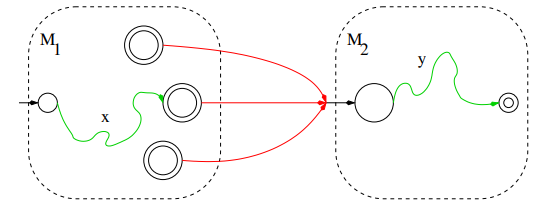
\includegraphics[scale=0.7]{concatenation}
\end{center}
The result is not a DFA because of the red transitions
\section{Non-deterministic Finite Automaton (NFA)}
A NFA is a 5-tuple $(Q,\Sigma, \delta, q_0, F)$, where
\begin{enumerate}
	\item Q is a finite set of states
	\item $\Sigma$ is a finite alphabet
	\item $\delta: Q\times (\Sigma\cup \{\epsilon\})\rightarrow \mathscr{P}(Q)$ is the transition function
	\item $q_0\in Q$ is the start state, and
	\item $F\subseteq Q$ is the set of accept states
\end{enumerate}
\subsection{Computation of a NFA}
Let $M=(Q,\Sigma, \delta, q_0, F)$ be a NFA and $w=w_1w_2...w_n$ be a word over $\Sigma\cup \{\epsilon\}$\\
\textbf{Important remark}: $\epsilon$'s can be freely added inside the actual word $\in\Sigma^*$\\
\\
M accepts w if there exists a sequence of states $r_0,r_1,r_2,...,r_n$ satisfying the following conditions:
\begin{enumerate}
	\item $r_0=q_0$
	\item $r_{i+1}\in \delta(r_i,w_{i+1})$ for every $0\leqslant i\leqslant n-1$ and
	\item $r_n\in F$
\end{enumerate}
\textbf{DFA} - There is a unique computation (path). It either accepts or rejects\\
\textbf{NFA} - There are, in general, many computational paths. The NFA accepts if at least one computation accepts. The NFA rejects only if all the computations reject.
\section{Converting a NFA into a DFA}
At any time there are a number of possible states the NFA computation can be into. As the DFA needs to keep track of all of these, the DFA's states will correspond to subsets of the NFA's-state set. The transition function of the DFA can then be defined as shown below:
\begin{center}
	\includegraphics[scale=0.7]{"NFA to DFA"}
\end{center}
Let $N=(Q,\Sigma, \delta, q_0, F)$ be a NFA recognising some language L (assume that L has no $\epsilon$ transitions). We shall construct a DFA $M=(Q',\Sigma, \delta', q_0', F')$ that recognises the same language L as follows
\begin{enumerate}
	\item $Q'=\mathscr{P}(Q)$
	\item For $R\in Q'$ and $a\in \Sigma$ let
	\[
	\delta^{\prime}(R, a)=\{q \in Q | q \in \delta(r, a) \text { for some } r \in R\}
	\]
	Equivalently
	\[
	\delta^{\prime}(R, a)=\bigcup_{r \in R} \delta(r, a)
	\]
	\item $q_0'=\{q_0\}$
	\item \(F^{\prime}=\left\{R \in Q^{\prime} | \exists r \in R r \in F\right\}\)
\end{enumerate}
Let us take care of $\epsilon$-transitions. For $R\subseteq Q$ (same as $R\in Q'$) let\\
$$E(R)=\{q | q \text { is reachable from } R \text { through a number of } \varepsilon \text { -transitions. }\}$$
Modify the construction as follows
\begin{enumerate}
	\item $Q'=\mathscr{P}(Q)$
	\item For $R\in Q'$ and $a\in \Sigma$ let
	\[
	\delta^{\prime}(R, a)=\{q \in Q | q \in E( \delta(r, a)) \text { for some } r \in R\}
	\]
	Equivalently
	\[
	\delta^{\prime}(R, a)=\bigcup_{r \in R} E(\delta(r, a))
	\]
	\item $q_0'=E(\{q_0\})$
	\item \(F^{\prime}=\left\{R \in Q^{\prime} | \exists r \in R r \in F\right\}\)
\end{enumerate}
\section{Closure under regular operations}
Union
\[
A \cup B=\{x | x \in A \text { or } x \in B\}
\]
\begin{center}
	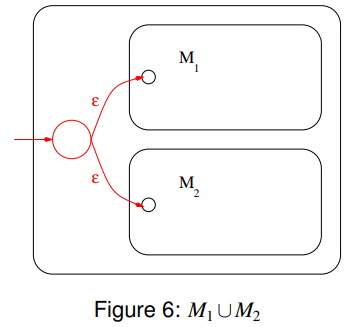
\includegraphics[scale=0.7]{Union}
\end{center}
Concatenation
\[
A \circ B=\{x y | x \in A \text { and } y \in B\}
\]
\begin{center}
	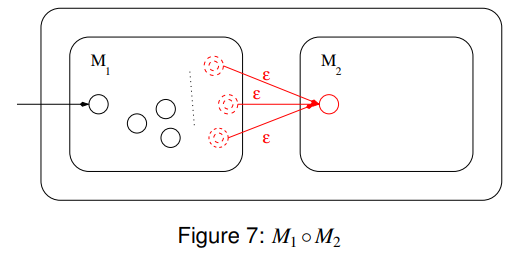
\includegraphics[scale=0.7]{Concatenation}
\end{center}
Star
\[
A^{*}=\left\{x_{1} x_{2} \ldots x_{k} | k \geq 0 \text { and } x_{i} \in A \text { for every } i, 1 \leq i \leq k\right\}
\]
\begin{center}
	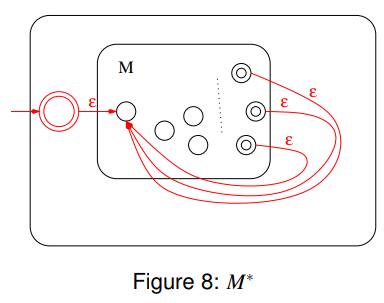
\includegraphics[scale=0.7]{Star}
\end{center}
\section{Equivalence of FA and Regular Expressions}
\textbf{Theorem} - A language is regular iff some regular expression describes it\\
\textbf{Proof}\\
$\Leftarrow$ Given a RE R, construct a NFA that recognises L(R) - this can be done by structural induction\\
\\
\textit{Base case} - All initial REs can be implemented by NFAs\\
\textit{Inductive step} - We have already proven that the class of regular languages is closed under regular operations\\
\\
$\Rightarrow$ Given a DFA M, construct a RE that recognises L(M)

\section{Generalised Non-deterministic Finite Automaton (GNFA)}
\begin{enumerate}
	\item A single start state with no incoming edges
	\item A single accept state with no outgoing edges
	\item Every transition is labelled with a regular expression
\end{enumerate}
-\begin{center}
	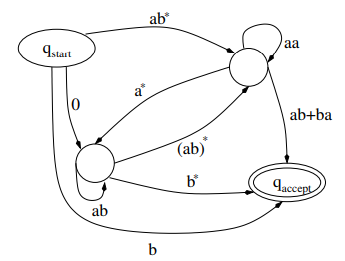
\includegraphics[scale=0.7]{GNFA}
\end{center}
\section{DFA into RE}
\begin{enumerate}
	\item Convert the given n-state DFA(NFA) into an equivalent n+2 state GNFA
	\begin{center}
		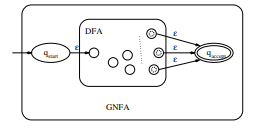
\includegraphics[scale=0.7]{DFA_to_RE}
	\end{center}
	\item Eliminate all internal states of the GNFA one by one, while preserving the language recognised by the automaton
	\begin{center}
		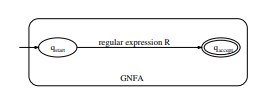
\includegraphics[scale=0.7]{DFA_to_RE1}
	\end{center}
	\item We are done, as $L(R)=L(DFA)$
\end{enumerate}
\section{Internal state elimination}
Pick an internal state r for elimination\\
For every two states u and v $u\neq r\neq v$, do the following
\begin{center}
	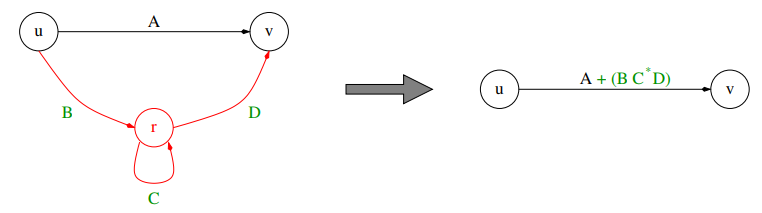
\includegraphics[scale=0.7]{Elimination}
\end{center}
\section{Non-regular languages}
How do we prove that a given language N is not regular?
\begin{itemize}
	\item Can't be recognised by DFA: assume that there is a DFA that recognises N and then use an adversary argument against that DFA in order to get a contradiction
\end{itemize}
\section{Pumping Lemma}
For every regular language L, there is a number p (called "pumping length" of L) such that every word $w\in L$ of length at least p can be divided into three parts $w=xyz$, satisfying the following conditions:
\begin{enumerate}
	\item $xy_iz\in L$ for every $i\in \mathbb{N}$ (in particular $xz\in L$ as one can take $i=0$)
	\item $y$ is a non empty string
	\item The length of the string $xy$ is not greater than p
\end{enumerate}
\textbf{Proof} Let $M=(Q,\Sigma, \delta, q_0, F)$ be a DFA that recognises L, and let us set the pumping length p to be the number of states in M: $p=|Q|$\\
Consider the computation of M on the word $w=w_1w_2...2_n$ (where $n\leqslant p$)
\[
q_{0}=r_{0} \rightarrow^{w_{1}} \rightarrow r_{1} \rightarrow r_{2} \rightarrow r_{2} \rightarrow \cdots \cdots \cdots r_{n-1} \rightarrow r_{n} \in F
\]
Let i be the first moment in time where we see a repetition in the states $r_0,r_1,r_2,...,r_n$ (such an i exists by the pigeon hole principle as $n+1>p$) Then we can set $x=w_1w_2...w_j$, $y=w_{j+1}..w_i$ and $z=w_{i+1}...w_n$\\
\\
It is now straightforward to check that all three conditions are met
\section{DFA Minimisation}
An algorithm that "minimises" any given DFA, i.e. finds an equivalent DFA with the minimal number of states. It answers at once the following important questions
\begin{enumerate}
	\item What is the smallest (in terms of number of states) DFA that recognises the same language?
	\item Given two DFAs, do they recognise the same language
\end{enumerate}
\subsection{Outline of the algorithm}
\begin{enumerate}
	\item Remove all the states that are not reachable from the start state
	\item Contract a set of states that are equivalent into a single state
\end{enumerate}
Two states, s and t, are equivalent if any word w, which is accepted when starting from s, is accepted when starting from t and vice versa.
\subsection{Equivalent and Distinguishable states}
\textbf{Extended Transition Function}: Let a DFA $M=(Q,\Sigma, \delta, q_0, F)$ be given and let $\hat{\delta}: Q\times \Sigma^8\rightarrow Q$ be defined as
\[
\begin{array}{c}
{\hat{\delta}(s, \varepsilon)=s} \\
{\hat{\delta}\left(s, w_{1} w_{2} \ldots w_{n}\right)=\hat{\delta}\left(\delta\left(s, w_{1}\right), w_{2} \ldots w_{n}\right)}
\end{array}
\]
for every state s and every word $w_1w_2...w_n$\\
\textbf{Equivalent states}: Two states s and t are equivalent if
\[
\left\{w \in \Sigma^{*} | \hat{\boldsymbol{\delta}}(s, w) \in F\right\}=\left\{w \in \Sigma^{*} | \hat{\boldsymbol{\delta}}(t, w) \in F\right\}
\]
Otherwise, s and t are distinguishable, i.e. there is a witness word u such that either \(\hat{\delta}(s, u) \in F, \hat{\delta}(t, u) \notin F\) or \(\hat{\delta}(s, u) \notin F, \hat{\delta}(t, u) \in F\)
\section{Team-Splitting Algorithm}
Best explained in terms of teams of players (sets of states) that pass balls of different colours (input symbols via transmissions)\\
\\
\textbf{Start}: Disqualify useless players (states that are unreachable from the start state)\\
\\
\textbf{Round 0}: Start with two teams, one consisting of all the accept states and the other consisting of all the non-accept states. Set $i:=1$\\
\\
\textbf{Round i}: For every team $S\in \mathscr{P}(Q)$ and every colour $a\in \Sigma$ check if all players from S agree on passing an a-ball. If not, split the team S into the maximal sub-teams that agreed, set $i:=i+1$ and go to round i\\
\\
\textbf{End}: Return the teams as sets of equivalent states
\subsection{Correctness of the algorithm}
\textbf{Proposition}: The Team-Splitting algorithm terminates\\
\\
\textbf{Proof}: There cannot be more than $n-1$ splits (where n is the number of players)\\
\\
\textbf{Proposition}: Every two players that are in the same team in the end are equivalent\\
\\
\textbf{Proof}: Pick any sequences of passes (a word) and prove, by induction of its length, that it can't tell the two players apart\\
\\
\textbf{Proposition}: Every two players that have been split at some round can't be equivalent\\
\\
\textbf{Proof}: Induction on the round number. The inductive step - a proof by contradiction.
\section{Equivalence and Isomorphism of DFAs}
Two see if two DFAs recognise the same language put them together, apply the minimisation algorithm as if they were as single automaton, and see whether the two start states are equivalent\\
\\
\textbf{Corollary}: If $M_1$ and $M_2$ are two minimal DFAs that recognise the same language, the minimisation algorithm always produces a bijection between the (equivalent) states of $M_1$ and $M_2$. We say that $M_1$ and $M_2$ are isomorphic\\
\\
\textbf{Proof}: Build the bijection starting from the two start states\\
\\
\textbf{Theorem}: The team splitting algorithm finds the minimal DFA equivalent ot the original one\\
\\
\textbf{Proof}: By first arguing that the DFA produced by the algorithm is equivalent to the minimal one, and then observing that the former can't have unreachable or equivalent states, so it must be isomorphic to the latter 
\end{document}